\documentclass[tikz,border=6pt]{standalone}
\usepackage{pgfplots}
\pgfplotsset{compat=1.18}
\definecolor{curveblue}{RGB}{37,99,235}
\definecolor{rootgreen}{RGB}{5,150,105}
\definecolor{vertexviolet}{RGB}{124,58,237}
\definecolor{axisgray}{RGB}{100,116,139}
\begin{document}
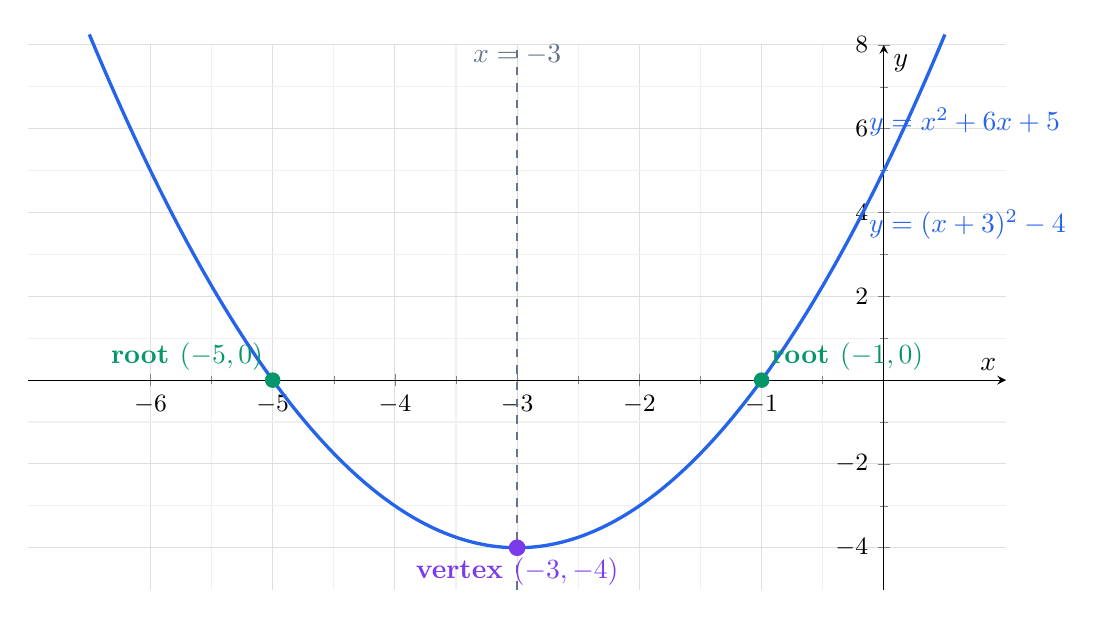
\begin{tikzpicture}
\begin{axis}[
  width=14cm,
  height=8.5cm,
  axis lines=middle,
  xlabel={$x$},
  ylabel={$y$},
  xmin=-7,
  xmax=1,
  ymin=-5,
  ymax=8,
  xtick={-6,-5,-4,-3,-2,-1,0},
  ytick={-4,-2,0,2,4,6,8},
  grid=both,
  minor tick num=1,
  major grid style={draw=gray!25},
  minor grid style={draw=gray!12},
  tick label style={font=\small},
  label style={font=\bfseries},
  samples=240,
  clip=false,
]
\addplot[curveblue, very thick, domain=-6.5:0.5] {x^2 + 6*x + 5};
\addplot[axisgray, dashed, thick] coordinates {(-3,-5) (-3,8)};
\addplot[rootgreen, only marks, mark=*, mark size=2.6pt] coordinates {(-5,0) (-1,0)};
\addplot[vertexviolet, only marks, mark=*, mark size=2.8pt] coordinates {(-3,-4)};
\node[anchor=south west, text=curveblue, font=\bfseries] at (axis cs:-0.2,5.6) {$y=x^2+6x+5$};
\node[anchor=north west, text=curveblue, font=\bfseries] at (axis cs:-0.2,4.3) {$y=(x+3)^2-4$};
\node[anchor=south east, text=rootgreen, font=\bfseries] at (axis cs:-5,0) {root $(-5,0)$};
\node[anchor=south west, text=rootgreen, font=\bfseries] at (axis cs:-1,0) {root $(-1,0)$};
\node[anchor=north, text=vertexviolet, font=\bfseries] at (axis cs:-3,-4) {vertex $(-3,-4)$};
\node[anchor=south, text=axisgray, font=\bfseries] at (axis cs:-3,7.3) {$x=-3$};
\end{axis}
\end{tikzpicture}
\end{document}
